\graphicspath{{../images/intro/}}
\chapter{Постановка задачи и обзор существующих методов}
%Чтобы разрабатывать современные эффективные лекарства, надо учитывать процессы, происходящие в клетках. Большинство важных процессов построено на взаимодействии белков с другими белками или малыми молекулами - лигандами.


%В моей работе рассматривается один из простейших случаев белок-белкового взаимодействия, при котором оценивается взаимодействие двух цепочек белка. За счет химических связей и электростатических взаимодействий они связываются между собой и образуют комплекс. 


\section{Белок-белковое взаимодействие. Определения}
% - что такое белки
% - из чего состоят
% - что такое поверхность белка
% - информация о вторичной структуре 
%(мб сказать что такое вторичная структура белка?  вынести во введение или первую главу)
%Зачастую являясь результатом несинонимичной замены одного нуклеотида, точечная мутация одной аминокислоты может приводить к масштабным последствиям: так, например,
%\todo{дописать}

%\todo {вообще здесь должно быть не про точечные мутации, а какие-то общие слова. Блаблабла, дизайн лекарств, блаблабла. и при чем тут белки.}
%\subsection{Определения}
Когда-то давно на Земле зародилась жизнь. Ее основой стали аминокислоты -- небольшие органические молекулы. Каждая аминокислота состоит из двух частей: основной цепи, одинаковой для всех аминокислот, и боковой цепи (боковую цепь также называют радикалом, у каждой аминокислоты она своя). Основная цепь состоит из аминогруппы ($NH_2$), карбоксильной группы ($COOH$), и соединяющего их вместе атома углерода, на который ,,подвешена'' боковая цепь. 

В свою очередь, белок образован одной или несколькими последовательностями, или цепочками, таких аминокислот (см. рисунок \ref{fig:aa3_1}).

\begin{figure}[h]
%\resizebox{0.9\textwidth}{!}{
%\input{aa3_5.tex}
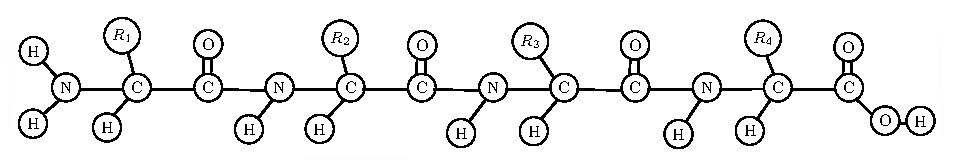
\includegraphics[width=\linewidth]{aa3_1.eps}
%}
\caption{\small{Схематичное изображение первичной структуры белка -- цепочки аминокислот, соединенных ковалентными связями между амино- и карбоксильными группами. Показана основная цепь белка; радикалы, отличающие аминокислоты одну от другой, условно обозначены $R_1$, $R_2$, $R_3$ и $R_4$. }}
\label{fig:aa3_1}
\end{figure}

Последовательность аминокислот в цепочке определяет первичную структуру белка. Когда мы рассматриваем положение цепочки в пространстве, то речь идет о вторичной и третичной структурах. Наконец, несколько цепочек, объединяясь в пространстве, образуют четвертичную структуру.

Ключевое отличие между первичной, вторичной, третичной и четвертичной структурами -- виды химических связей, с помощью которых они образованы: так, например, первичная структура белка образуется за  счет сильных ковалентных связей, образующихся между аминогруппой и карбоксильной группой двух соседних аминокислот.

%%\newpage
Когда мы рассматриваем несколько цепочек в составе одного белка или несколько белков, образующих комплекс, мы говорим о \textbf{белок-белковом взаимодействии}.
Чем меньше свободная энергия Гиббса $\triangle\,G$ этого комплекса по сравнению с суммарной энергией цепочек, тем он более стабилен. Говорят, что в таких случаях лучше \textbf{сцепленность}\footnote{Можно трактовать понятие ,,сцепленность'' в топологическом смысле -- для этого вводят в рассмотрение искусственные характеристики для ее оценки (как, например, это сделано в работах \cite{ialign, pcalign}), но мы будем понимать под ,,лучшей сцепленностью'' именно большее изменение  свободной энергии комплекса как более естественную численную характеристику, достаточную для решения задачи, поставленной в рамках данной работы. } цепочек. 



%\textbf{Вторичная структура} задается укладкой цепочки аминокислот в пространственные структуры, \textbf{третичная структура} - расположением этих структур в пространстве в случае, когда белок содержит только одну цепь.

%Когда белок состоит из нескольких цепей, говорят о его \textbf{четвертичной структуре}.

Область пространства вблизи обоих белков, образующих комплекс, называют \textbf{интерфейсом} белок-белкового взаимодействия (схематичное изображение приведено на рисунке \ref{fig:ppi}). 


\begin{figure}
%\resizebox{0.9\textwidth}{!}{
%\input{aa3_5.tex}
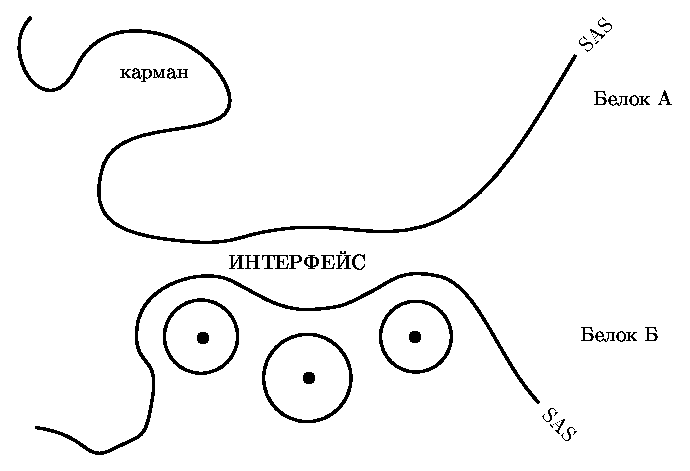
\includegraphics[width=\linewidth]{ppi.eps}
%}
\caption{\small{Схематичное изображение пары взаимодействующих белков, формирующих комплекс. Показаны фрагменты рельефа молекулярной поверхности, доступной для растворителя (на рисунке линия, обозначенная SAS - от англ solvent accessible surface), сферы Ван-дер-Ваальса для нескольких атомов одного из белков -- для упрощения восприятия  приведено схематичное изображение в проекции на плоскость. }}
\label{fig:ppi}
\end{figure}


Также, когда говорят о взаимодействии, используют понятие \textbf{поверхностей}. Для этого представляют молекулу в виде объединения шаров, центры которых совпадают с центрами образующих ее атомов, а радиусы соответствуют радиусам Ван-дер-Ваальса. Граница областей, на которые разбивается пространство, из которого исключено такое объединение шаров, называется \textbf{поверхностью Ван-дер-Ваальса} для этой молекулы. Дополнительно вводят понятие \textbf{молекулярной поверхности} -- всех возможных положений центра сферы с фиксированным радиусом, касающейся поверхности Ван-дер-Ваальса данной молекулы. В случае, когда радиус сферы совпадает с радиусом сферы, в которую можно вписать молекулу воды, такую поверхность называют \textbf{поверхностью, доступной для растворителя} (на рисунке \ref{fig:ppi} обозначена аббревиатурой SAS -- от англ. solvent accessible surface).

Если внешняя поверхность белка в каком-то месте является вогнутой, а не выпуклой, то говорят, что это карман. 

%\subsection{Белки и энергия}
%С точки зрения химии, разным видам структуры соответствуют разные виды химических связей и электростатических взаимодействий.



%Свободная энергия связи, обозначаемая \ddG, определена как разность $\vartriangle\!G_{mut} - \vartriangle\!G_{wt}$ , где $\vartriangle\!G_{wt}$ и $\vartriangle\!G_{mut}$ -- изменения свободной энергии Гиббса для немодифицированного белка и его подвергнутой точечному мутагенезу версии (alanine-mutated protein).
%\newpage
%\subsection{Поверхность белка как его энергетический фронт}
%\subsection{Энергетически значимые аминокислотные остатки}
%Понятие энергетически горячего аминокислотного остатка тесно связано с понятием интерфейса взаимодействия белков. Для того, чтобы понять, в каких регионах следует в первую очередь искать ЭГАО, необходимо понимать важные свойства интерфейсов белок-белкового взаимодействия и областей связывания белков:
%\subsection{Белок-белковое взаимодействие}
%\todo{переделать}




%Ответить нам поможет \textbf{аланиновое сканирование} (аланиновый мутагенез).

\newpage
\section{Аланиновое сканирование}
При разработке лекарств на основе моноклональных антител часто возникает необходимость улучшить структуру существующего белка, оценить, насколько хорошо он присоединяется к антигену, убедиться, что при этом случайная точечная мутация антигена не приведет к сильному снижению эффективности лекарства, или, наоборот, оно не будет связывать другие белки, выполняющие важные функции в клетке.

Простейший из методов, которые позволяют получить ответы на эти вопросы -- \textbf{аланиновое сканирование} (аланиновый мутагенез). 

Можно провести небольшое изменение -- например, заменить одну аминокислоту в цепочке -- и посмотреть, не произойдет ли при этом существенного изменения свободной энергии Гиббса, не приведет ли это к усилению или ослаблению сцепленности между цепочками комплекса.

Но как выбирать аминокислоту, на которую проводить замену? Всегда ли стоит перебирать все аминокислоты в одной и той же позиции в цепочке?

Экспериментально было показано~\cite{alascan2001}, что достаточно заменить аминокислоту на аланин, чтобы понять, является ли она энергетически значимой при оценке взаимодействия цепочек, или нет. А затем, если изменение энергии комплекса  оказывается существенным, перебрать все оставшиеся аминокислоты в данной позиции и определить, какая замена является экстремальной.

Понять, почему для точечной мутации выбирают именно аланин, может помочь рисунок \ref{fig:aminoacids}, на котором в центре изображена химическая формула аланина, окруженная формулами других аминокислот.

\begin{figure}
 \resizebox{!}{0.9\textwidth}{
 \ttfamily
 \footnotesize
 \aapicture
 }
\caption{\small{Химические формулы аминокислот (без учета хиральности), в центре -- аланин; черным цветом в формулах показаны фрагменты аминокислот, формирующие основную цепь белка; красным цветом показаны фрагменты боковых цепей, которые подвергаются мутации при аланиновом сканировании. Стрелками на схеме показано направление мутации на первом шаге аланинового сканирования -- т.е. в направлении к аланину от всех прочих аминокислот. }}
\label{fig:aminoacids}
\end{figure}

Как видим, аланин -- аминокислота с коротким радикалом, относительно легкая, химически нейтральная; может участовать в формировании как $\alpha$-спиралей, так и $\beta$-листов -- поэтому замена аминокислоты на аланин в этих элементах вторичной структуры не приводит к существенному нарушению их формы.

Можно заметить, что у глицина (на рисунке \ref{fig:aminoacids} эта аминокислота подписана трехбуквенным англоязычным сокращением Gly) боковая цепь отсутствует, или, точнее, представлена только одним атомом углерода (его обозначают $C_\alpha$, или $\alpha$-углеродом), на который у других аминокислот боковая цепь ,,подвешена'' к основной цепи. Почему не проводят глициновое сканирование? Все дело в том, что за счет отсутствия боковой цепи, участок с глицином обладает большей гибкостью, чем остальные, результат замены аминокислоты на глицин может значительно отличаться от замены на другие аминокислоты, его сложнее интерпретировать.

Если $\alpha$-углерод является частью основной цепи, то $\beta$-углерод уже является частью боковой цепи (радикала), его положение определяется пространственным положением основной цепи. По нему уже можно понять,  как будет повернута модифицированная боковая цепь, при этом радикал аланина, кроме $\beta$-углерода, не содержит других атомов, которые сделали бы его тяжелее, полярнее, возможно, гидрофобнее, и тем самым усложнили дальнейший анализ.
%На рисунке \ref{fig:aminoacids} части аминокислот, которые образуют основную цепь цепочки белка и определяют положение цепи в пространстве, показаны красным цветом Замена аминокислоты на  на аланин Alanine (Ala) has propensity to form alpha helices but can also occur in beta sheets and is generally equivalent to simply truncating a side chain back to the beta carbon, which is the first side chain atom. The beta carbon position depends upon the backdone dihedral angles of the polypeptide so is really part of the main chain structure of the protein. Thus, alanine is generally an accepted single residue first choice for mutational scanning because it retains the beta carbon but no other side chain chemistry. Glycine which removes the beta carbon is unusually flexible and can take on polypeptide backbone conformations generally not allowed by other amino acids, so mutation to glycine will cause flexibility and possible conformational changes convoluted with the effects of removing the side chain atoms making interpretation more complex than for Ala. Replacing side chains with larger, more constrained (such as branched beta carbon side chains of valine and Isoleucine), more polar, differently charged, or more hydrophobic atoms may all cause changes in structures and conformation along with the side chain chemistry thereby complicating analyses of results more than Ala.

%\begin{wrapfigure}{RT}{0.3\textwidth}
%\resizebox{0.2\textwidth}{!}{
%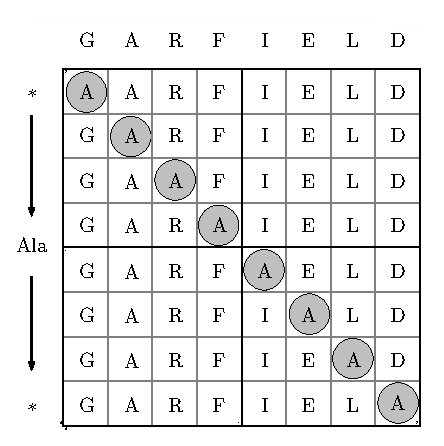
\includegraphics{ala_scan.eps}
%}
%\end{wrapfigure}
%\newpage
\subsection{Аланиновое сканирование in vitro/in vivo}
Первоначально аланиновое сканирование появилось как лабораторный, химический метод (in vitro/in vivo), с вытекающими отсюда свойствами:
\begin{itemize}
\item Большое пространство поиска: для того, чтобы определить энергетически значимые аминокислоты, требовалось проверить все. В случае антител, только тяжелые цепи содержат порядка 450-550 аминокислот.
\item Сложность синтеза библиотек: в каждом индивидуальном случае необходимо выбрать метод для синтеза, получить и разделить образцы с точечными мутациями в каждой из позиций цепочки. В отдельных случаях необходимо проводить рефолдинг полученных точечно-модифицированных белков.
\item Как следствие, высокая стоимость - как в денежном, так и во временном эквиваленте.
\end{itemize}

Создание библиотеки белков с точечными мутациями in vivo позволяет упростить получение модифицированных пептидов, но оно доступно для ограниченного числа белков ~\cite{alascan2001}.

У экспериментального аланинового  сканирования есть один существенный ,,плюс'' -- оно позволяет выявить  аминокислоты, которые существенно влияют на функцию, стабильность или форму белка в клетке и оценить такое влияние с небольшой погрешностью. Причем результат такого эксперимента будет близок к тому, что произойдет в клетке. 

Чтобы сократить затраты на аланиновое сканирование в лаборатории, применяют теоретическое, компьютерное моделирование аланинового сканирования, обозначенное в теме данной работы как \textbf{ala-scan in silico} -- в противовес экспериментальному лабораторному аланиновому сканированию. Обычно его используют для выбора потенциально важных аминокислот, но, разумеется, результаты проверяют в лаборатории, создавая экспериментальную библиотеку образцов с мутациями уже не по всем позициям, а только по выбранным in silico, сокращая тем самым стоимость эксперимента.

Посмотрим, каким образом происходит аланиновое сканирование in silico.
%уточнить цифру \newpage
\subsection{Аланиновое сканирование in silico: решаемые задачи и границы применимости}

Компьютерное моделирование аланинового сканирования позволяет удешевить разработку лекарственных средств: с его помощью решают различные задачи, возникающие при разработке современных, высокотехнологичных лекарств. С помощью модификации всего одной аминокислоты можно оценить специфичность разрабатываемого лекарства, синтезировать новый, не запатентованный белковый препарат, не отличающийся по эффективности от уже запатентованных, или, например, убедиться в том, что разрабатываемый препарат не взаимодействует с важными функциональными элементами клетки. 


Если при экспериментальном аланиновом сканировании можно относительно точно оценить, насколько изменилась свободная энергия комплекса после замены одной аминокислоты, то при компьютерном моделировании приходится применять различные методы для грубой оценки этого изменения. Еще одна задача, которую необходимо решать - правильно (в смысле реалистичности происходящего изменения) проводить рефолдинг -- пересборку белка после точечной мутации.

Так, например, для уточнения структуры, которую примет цепочка с точечной мутацией и исследуемый комплекс в целом, используются различные методы -- от приближенных, но универсальных, таких как метод Монте-Карло на решетке, до точных, но специфичных для конкретного белка и условий среды, таких как моделирование с помощью методов молекулярной динамики.

Основная цель таких методов -- достоверно оценить, насколько и в какую сторону изменится изменение свободной энергии Гиббса \ddG комплекса при внесении точечной мутации в одну из цепочек.
%$$\Delta\Delta G_{bind} = (\Delta G_{M complex} - \Delta G_{M_A} - \Delta G_{M_B}) - (\Delta G_{WT complex} - \Delta G_{WT_A} - \Delta G_{WT_B})$$

В данной работе используется протокол аланинового сканирования из пакета rosetta с немодифицированной функцией свободной энергии~\cite{kortemme2002}, которая позволяет эффективно предсказать изменение энергии комплекса в случаях, когда  взаимодействие с водой не учитывается.

Детали реализации протокола не приводятся, поскольку их рассмотрение не является основной целью данной работы.
%\todo{сказать, что в данной работе используется протокол из rosetta (мб привести картинку про реальную ddG и in silico функцию изменения энергии), сцепленность цепочек оценивается в смысле изменения энергии, применяемый в протоколе метод монте-карло лежит за пределами работы (кроме того, является относительно хорошо изученным, в ходе работы никакие модификации в сам метод или функцию оценки ddG не вносились), поэтому не приводится. }



%Поэтому \textbf{цель} моей \textbf{работы} - построить биологически обоснованный алгоритм выбора аминокислот для компьютерного аланинового сканирования.

\section{Формулировка задачи}
Рассмотрим белок-белковый комплекс, образованный двумя цепочками белка. В условиях, когда взаимодействие с водой не учитывается, выберем одну из цепочек. 

Цель работы -- предложить алгоритм поиска протяженных регионов (позиций аминокислот в цепочке), определяющих специфичность по отношению ко второй цепочке такого комплекса.

Для построения такого алгоритма необходимо решить ряд задач:

1. Определить признаки, которые определяют энергетическую значимость аминокислот.

2. Выбрать среди признаков легко алгоритмизуемые.

3. Предложить алгоритм выбора аминокислот, формирующих протяженные регионы, определяющие специфичность по отношению ко второй цепочке комплекса. Написать программную реализацию.

4. Провести анализ полученного алгоритма: для этого необходимо определить средства, с помощью которых будет проводиться такой анализ, а также проинтерпретировать полученные результаты.
%\newpage
\section{Существующие решения}


%Стандартные методы выбора аминокислот для аланинового сканирования in silico
Применяют два принципиально разных подхода~\cite{hotspots2012rev}, с помощью которых выбирают аминокислоты для аланинового сканирования: 
\begin{itemize}
\item поиск аминокислот вблизи интерфейса взаимодействия цепочек;
\item предсказание позиций энергетически важных аминокислот по уже накопленной информации об интерфейсах и результатам экспериментального аланинового сканирования.
\end{itemize}


При использовании первого метода выбираются аминокислоты, находящиеся в области интерфейса взаимодействия цепочек. При этом выбор происходит точечно, регион может быть выбран не целиком, в нем могут быть пропуски и “дыры”. Такое произойдет, например, если в области интерфейса белок-белкового взаимодействия расположен карман.

При использовании второго метода учитывается информация из имеющихся баз данных с результатами экспериментального аланинового сканирования для предсказания возможных позиций, в которых следует искать энергетически значимые аминокислоты. Такой класс методов позволяет предсказать значимые аминокислоты при наличии информации по похожим структурам, он плохо работает при отсутствии такой информации. Кроме того, известно, что энергетически значимые аминокислоты специфичны по отношению к взаимодействующим компонентам комплекса, поэтому предсказание может не дать хороших результатов.

Оценим эффективость каждого из этих методов.

%\newpage
\subsection{Выбор аминокислот вблизи интерфейса взаимодействия с отсечкой по расстоянию}

Способ фильтрации аминокислот, при котором выбираются для последующей мутации только те из них, которые находятся вблизи интерфейса взаимодействия компонент исследуемого комплекса, биологически обоснован. Во-первых,  консервативные в смысле эволюции белков аминокислоты являются таковыми потому, что вносят важный вклад в сохранение функций, стабильности или формы белка. Они же часто оказываются в области интерфейса взаимодействия белков. Во-вторых, энергетически важные аминокислоты обычно специфичны по отношению к взаимодействующему комплексу белков, так же, как и интерфейс такого взаимодействия, поэтому эти понятия часто не различают.

Способ выбора аминокислот с  отсечкой по расстоянию от интерфейса взаимодействия ~\cite{kortemme2004} -- универсален, он может использоваться при дизайне белков de novo, то есть в ситуациях, когда белок синтезируется впервые, экспериментальное аланиновое сканирование эволюционно близких к нему белков ранее не проводилось. 

Как правило, в качестве величины отсечки берут величину порядка  4-8 \AA{}. В  Rosetta Alascan Protocol~\cite{kortemme2004} используется усложнение: дополнительно рассматриваются аминокислоты, $\beta$-углерод которых после формирования комплекса в шаре определенного фиксированного радиуса содержит существенно больше атомов $\beta$-углерода, чем содержал до этого.
%\newpage
\subsection{Контрпример}
%\newpage
Описанный подход не всегда эффективен, поскольку он не всегда выявляет энергетически значимые аминокислоты. Покажем это с помощью простого компьютерного эксперимента:
\begin{enumerate}
\item Рассмотрим базу данных с информацией о результатах эспериментов по аланиновому сканированию белков ASEdb~\cite{asedb2001}. Найдем объекты с корректными ссылками на записи в Protein Data Bank ~\cite{rcsb}.
\item Среди всех таких объектов найдем те, в которых есть аминокислоты, мутация которых приводит к существенному изменению свободной энергии комплекса. Существенным будем считать изменение, не меньшее, чем 1 килокалория на моль.
\item Посмотрим, всегда ли такие аминокислоты удалены от интерфейса в пределах стандартно используемой отсечки (в качестве примера возьмем расстояние, не превышающее 8 \AA{}).
\end{enumerate}

Результат работы скрипта для PyMOL, отображающего результаты этого эксперимента для одной из записей в ASEdb, показан на  рисунке \ref{fig:image7}.


\begin{figure}
%\resizebox{0.8\textwidth}{!}{
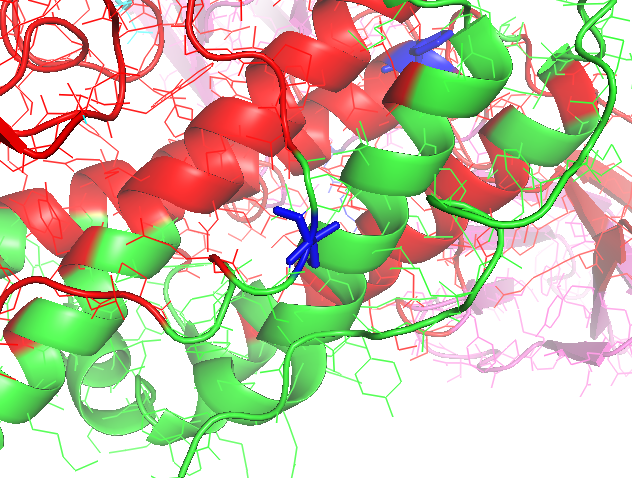
\includegraphics[width=\linewidth]{image7.png}
%}

\caption{\small{Снимок экрана, изображающий
белок-белковый комплекс, образованный  человеческим гормоном роста и рецептором человеческого гормона роста (идентификатор структуры в Protein Data Bank -- 3hhr). Красным цветом ,,окрашены'' аминокислоты одной из цепочек, атомы которых удалены от атомов парной цепочки, образующей  комплекс, не более, чем на 8 \AA{}. синим цветом ,,окрашены'' аминокислоты, точечное изменение которых приводит к существенному изменению свободной энергии комплекса.  }}
\label{fig:image7}
\end{figure}

Как видим, метод фильтрации аминокислот с отсечкой по расстоянию от интерфейса взаимодействия белков иногда упускает из рассмотрения аминокислоты, которые влияют на взаимодействие пары олигомеров, но при этом удалены от области интерфейса.

Такие аминокислоты, например, могут находиться в глубине карманов на поверхности одного из белков и, тем не менее, оказывать существенное влияние на стабильность белкового комплекса в целом \cite{pockets2004}.

%\newpage
\subsection{Предсказание энергетически значимых аминокислот}
%\todo{переделать}
%: аминокислоты отбираются исходя из имеющихся экспериментальных результатов аланинового сканирования, проводившихся на близких (в эволюционном смысле) последовательностях.

%Для эффективного поиска по гомологии необходимо иметь базу близких (ортологичных) структур, точную и содержащую всю информацию по результатам аланинового сканирования.

%Метод должен учитывать как данные о последовательности аминокислот в белках, так и каким-либо образом эксплуатировать пространственную структуру. В качестве примеров методов, учитывающих и то, и другое, можно привести ~\cite{svm1, svm2, hmmsvm}.

%\todo{в этом разделе надо сказать про различные инструменты, которые предсказывают хотспоты}

%Проводятся попытки классификации участков, 
%здесь можно ссылку на диссертацию студентки Фришмана

После того, как в лабораторной практике стали применяться различные техники эспериментального аланинового сканирования, появились и базы данных с его результатами ~\cite{asedb2001, bid2003}, но они фрагментированы, не всегда полны, разнородны (вероятно, это связано с тем, что данные собираются из разных источников и статей). Кроме того, данных в них не так много -- в силу приведенных выше свойств экспериментального точечного мутагенеза в лаборатории.

Например, если Protein Data Bank содержит информацию о большом количестве структур, с примерно одним и тем же форматом данных, то ASEdb представляет собой базу данных mysql и содержит информацию о 101 структуре, а BID доступна в виде набора wiki-страниц с информацией о конкретных белках или парах взаимодействующих цепочек.

Для того, чтобы получить рисунок \ref{fig:image7} из предыдущего параграфа, помимо просто изображения энергетически значимых аминокислот в PyMOL, пришлось дополнительно перебирать структуры из ASEdb и выбрать среди них те, которые содержат корректную ссылку на идентификатор структуры в Protein Data Bank, а также содержащую однозначную информацию о цепочке, которой принадлежит энергетически значимая аминокислота, подвергаемая мутации (в дампе с сайта ASEdb на момент обращения у некоторых записей название цепочки не было указано, кроме того, у некоторых записей позиция аминокислоты отсутствовала в соответствующем файле PDB -- этот факт можно объяснить тем, что с момента заполнения ASEdb структура в Protein Data Bank могла быть уточнена).

Единообразные и относительно сгруппированные данные представлены в наборе данных  \cite{kortemme_alascan_datasets}, который изначально был собран авторами компьютерного протокола аланинового сканирования в составе пакета Rosetta \cite{kortemme2002, kortemme2004} из разных источников для оценки его работы.

С появлением баз данных стал разрабатываться ряд теорий о структурной организации интерфейсов взаимодействия белков и предприниматься попытки ,,угадывать'' энергетически значимые аминокислоты или предсказывать изменение свободной энергии Гиббса при мутагенезе \cite{rev2}.

Некоторые из попыток предсказаний используют только данные последовательностей (например, ISIS - 
\cite{very_good}). Другие используют методы машинного обучения (APIS, KFC, MINERVA, HotPoint). Третьи учитывают и то, и другое (например, как сделано в работе \cite{hmmsvm}). При этом точность таких методов находится на уровне не более 82.1-83\% \cite{art2014,water}.


%Теория O-колец, утверждавшая, что энергетически значимые аминокислоты скорее всего являются таковыми за счет исключения растворителя. Ближайшие аминокислоты, которые образуют O-кольцо, нужны для того, чтобы отделять молекулы воды от энергетически значимых аминокислот \cite{orings}
Есть  работы, в которых авторы пытаются обобщить свойства энергетически значимых аминокислот и понять общие закономерности \cite{pockets2004, orings, loops2014}. В одной из последних таких работ \cite{loops2014} проводится попытка обобщить понятие ,,энергетически значимой аминокислоты'' до ,,энергетически значимой петли'' (,,горячей петли'').

%Например, появилась так называемая теория O-колец, утверждавшая, что энергетически значимые аминокислоты скорее всего являются таковыми за счет исключения растворителя. Ближайшие аминокислоты, которые образуют O-кольцо, нужны для того, чтобы отделять молекулы воды от энергетически значимых аминокислот
%
%The O-ring theory confirmed that occlusion of solvent is a necessary condition for highly energetic interactions (hot spots) and the residues on O-ring likely function to occlude bulk water molecules from binding hot spots.\cite{hotspots}\cite{water}
%\cite{  antibody, bloomberg, sdr_db}
\subsection{Выводы}
Задача поиска энергетически значимых аминокислот является труднорешаемой и трудноформализуемой, на текущий момент нет  инструментов, позволяющих предсказывать энергетически значимые аминокислоты с высокой точностью. 

